\documentclass[11pt,a4paper]{report} 
% Alternativ für doppelseitigen Ausdruck (nur bei > 60 Seiten sinnvoll)
% \documentclass[11pt,a4paper,twoside,openright]{report} 

% Deutsch
%\usepackage[german]{babel} % deutsch und deutsche Rechtschreibung
%\usepackage[english]{babel}
\usepackage[main=english, german]{babel}
\usepackage[utf8]{inputenc} % Unicode Text 
\usepackage[T1]{fontenc} % Umlaute und deutsches Trennen
\usepackage{textcomp} % Euro
\usepackage[hyphens]{url}
% statt immer Ab\-schluss\-ar\-beit zu schreiben
% einfach hier sammeln mit -. 
\hyphenation{Ab-schluss-ar-beit}
% Vorsicht bei Umlauten und Bindestrichen
\hyphenation{Ver-st\"ar-ker-aus-gang}
 % eigene Hyphenations, die für das Dokument gelten
\usepackage{amssymb} % Symbole
\usepackage{emptypage} % Wirklich leer bei leeren Seiten


%% Fonts, ein kompletter Satz an Optionen

% Times New Roman, gewohnter Font, ok tt und serifenlos
%\usepackage{mathptmx} 
%\usepackage[scaled=.95]{helvet}
%\usepackage{courier}

% Palatino mit guten Fonts für tt und serifenlos
\usepackage{mathpazo} % Palatino, mal was anderes
\usepackage[scaled=.95]{helvet}
\usepackage{courier}

% New Century Schoolbook sieht auch nett aus (macht auch tt und serifenlos)
%\usepackage{newcent}

% Oder default serifenlos mit Helvetica 
% ich kann es nicht mehr sehen ...
%\renewcommand{\familydefault}{\sfdefault}

\usepackage{microtype}

% Bilder und Listings
\usepackage{graphicx} % wir wollen Bilder einfügen
\usepackage{subfig} % Teilbilder
\usepackage{wrapfig} % vielleicht doch besser vermeiden
\usepackage{listings} % schöne Quellcode-Listings
% ein paar Einstellungen für akzeptable Listings
\lstset{basicstyle=\ttfamily, columns=[l]flexible, mathescape=true, showstringspaces=false, numbers=left, numberstyle=\tiny}
\lstset{language=python} % und nur schöne Programmiersprachen ;-)
% und eine eigene Umgebung für Listings
\usepackage{float}
\newfloat{listing}{htbp}{scl}[chapter]
\floatname{listing}{Listing}

% Seitenlayout
\usepackage[paper=a4paper,width=14cm,left=35mm,height=22cm]{geometry}
\usepackage{setspace}
\linespread{1.15}
\setlength{\parskip}{0.5em}
\setlength{\parindent}{0em} % im Deutschen Einrückung nicht üblich, leider

% Seitenmarkierungen 
\newcommand{\phv}{\fontfamily{phv}\fontseries{m}\fontsize{9}{11}\selectfont}
\usepackage{fancyhdr} % Schickere Header und Footer
\pagestyle{fancy}
\renewcommand{\chaptermark}[1]{\markboth{#1}{}}
%\fancyhead[L]{\phv \leftmark}
\fancyhead[L]{\phv \nouppercase{\leftmark}}
\fancyhead[R]{\phv \thepage}
% Unten besser auf alles Verzichten
%\fancyfoot[L]{\textsf{\small \kurztitel}}
\fancyfoot[C]{\ } % keine Seitenzahl unten
%\fancyfoot[R]{\textsf{\small Medieninformatik}}

% Theorem-Umgebungen
\newtheorem{definition}{Definition}[chapter]
\newtheorem{satz}{Satz}[chapter]
\newtheorem{lemma}[satz]{Lemma} % gleicher Zähler wie Satz
\newtheorem{theorem}{Theorem}[chapter]
\newenvironment{beweis}[1][Beweis]{\begin{trivlist}
\item[\hskip \labelsep {\textit{#1 }}]}{\end{trivlist}}
\newcommand{\qed}{\hfill \ensuremath{\square}}

% Quellen teilen
\usepackage{bibtopic} 

% Hochschule Logo, noch nicht perfekt
\usepackage{hsrmlogo}

% Spezialpakete
\usepackage{epigraph}
\setlength{\epigraphrule}{0pt} % kein Trennstrich

% damit wir nicht so viel tippen müssen, nur für Demo 
\usepackage{blindtext} 

% Zum Zeigen von Fehlern
\usepackage{soul}
\newcommand*\falsch{\st}

 % alle Pakete und Einstellungen

% Hier anpassen 
\newcommand{\welchethesis}{Bachelor}
% \newcommand{\welchethesis}{Master}
\newcommand{\thesisofwas}{of Science, Informatik - Technische Systeme}
\newcommand{\titel}{Study and implementation of a decentralized application that can provide
	permissionless financial services using an evm based blockchain}
%\newcommand{\kurztitel}{Template Abschlussarbeit}
\newcommand{\autor}{Mario Alberto Maita Orozco}
\newcommand{\datum}{30.06.2022} % Abgabedatum
\newcommand{\ort}{Wiesbaden}
\newcommand{\referent}{Prof.\ Dr.\ Eva-Maria Iwer}
\newcommand{\korreferent}{Prof.\ Dr.\ Marc-Alexander Zschiegner}

\begin{document}

\begin{titlepage}
  \begin{center}
    % Kopf der Seite
    \hsrmlogo[1]
    \parbox[b]{8cm}{Hochschule RheinMain \\
     Fachbereich Design Informatik Medien \\
     Studiengang Informatik - Technische Systeme}
    \vfill    
    {\LARGE Bachelor-Arbeit} \\[0.5cm]
    {\large zur Erlangung des akademischen Grades} \\[5mm]
    {\large \welchethesis\ \thesisofwas} \\[5mm]
    \rule{\textwidth}{1pt}\\[0.5cm]
    {\begin{spacing}{1.15} \LARGE \bfseries \titel \\ \end{spacing}}
    \rule{\textwidth}{1pt}    
    \vfill    
    \begin{tabular}{ll} % Mitte der Seite
      Vorgelegt von & \autor \\
      am & \datum \\
      Referent & \referent \\
      Korreferent & \korreferent
    \end{tabular}    
    \vfill
  \end{center}
\end{titlepage}
\cleardoublepage


% Erklärung gemäß den Allgemeinen Bestimmungen für Prüfungsordnungen
% der Paragraph schwankt, daher ohne Nennung einer Nummer
\thispagestyle{empty}
\section*{Erklärung gem. ABPO, Ziff. 4.1.5.4}
Ich versichere, dass ich die Bachelor-Arbeit selbständig verfasst und keine anderen als
die angegebenen Hilfsmittel benutzt habe.
´

\vspace{6em}
\noindent\begin{tabular}{p{0.37\textwidth}p{0.56\textwidth}}
\ort, \datum  & \rule{0.56\textwidth}{0.5pt}\\
              & \makebox[1cm]{\ } \autor
\end{tabular}

\vfill

\section*{Erklärung zur Verwendung der \welchethesis thesis}

Hiermit erkläre ich mein Einverständnis mit den im Folgenden aufgeführten
Verbreitungsformen dieser Bachelor-Arbeit:

\vspace{1em}
\noindent\begin{tabular}{|p{0.82\textwidth}|c|c|}
  \hline
  \textbf{Verbreitungsform} & \makebox[0.035\textwidth]{\textbf{Ja}} 
                            & \makebox[0.05\textwidth]{\textbf{Nein}} \\\hline
  Einstellung der Arbeit in die Hochschulbibliothek 
                         mit Datenträger   &  & $\times$ \\\hline
  Einstellung der Arbeit in die Hochschulbibliothek  
                         ohne Datenträger  & $\times$ & \\\hline
  Veröffentlichung des Titels der Arbeit im Internet  
                                           & $\times$ & \\\hline
  Veröffentlichung der Arbeit im Internet             
                                           &  $\times$  & \\\hline
\end{tabular}

\vspace{6em}
\noindent\begin{tabular}{p{0.37\textwidth}p{0.56\textwidth}}
\ort, \datum  & \rule{0.56\textwidth}{0.5pt}\\
              & \makebox[1cm]{\ } \autor
\end{tabular}
\cleardoublepage

 % Titelseite, Erklärungen, etc.

\begin{abstract} 
\LaTeX\ bietet Buchdruckqualität für jedermann.
Wir zeigen anhand dieses durch persönliche Präferenzen geprägtes Template, 
wie man Buchdruckqualität für eine Abschlussarbeit einfach erreichen kann.
Dazu werden beispielhaft Lösungen zu üblichen Fragestellungen im Dokument 
vorgestellt.
Zunächst benötigt man ein passendes \LaTeX\ System mit einigen 
installierten Erweiterungspaketen, das es erlaubt das Template zu 
übersetzen. 
Neben den grundlegenden For\-ma\-tie\-rungs\-möglich\-keiten mit \LaTeX\ wird 
insbesondere das Erstellen und Einbinden von Grafiken, Listings und 
mathematischen Formeln gezeigt.
Des Weiteren werden Literatur- und andere Verzeichnisse eingebunden.
Nicht zuletzt finden sich auch sachdienliche Hinweise zum
Schreiben und Zitieren von Literatur.
\end{abstract}

\tableofcontents
\newpage 

\chapter{Einführung} \label{chap:einf}
\epigraphhead[70]{\epigraph{Documentation is like sex: 
when it is good, it is very, very good; and when it is bad, 
it is better than nothing.}{\textit{Dick Brandon}}}


Der Ausdruck "`What you see is what you get"' (WYSIWIG) ist eine Drohung 
und kein Versprechen.
Trotzdem verwenden viele Autoren WYSIWIG-Werk\-zeuge, 
um ihre Dokumente zu erzeugen. 
Weitaus schlimmer ist, dass deutlich mehr Menschen die so erstellten 
Dokumente lesen müssen.
Zumindest für die eigene Abschlussarbeit sollte man es sich nicht entgehen 
lassen den Lesern etwas Schönes zum Lesen zu geben.
In erster Linie ist das natürlich der Inhalt. 
Aber das Auge isst mit und ein professionell gesetztes Dokument lässt den 
Inhalt in noch hellerem Licht erstrahlen.
Dazu bietet sich \LaTeX\ als Alternative zu Word \& Co. an.

Allerdings hat \LaTeX\ zugegebenermaßen eine steile Lernkurve. 
Man muss sowohl die Trennung von Struktur und Layout, als auch die grundlegend
andere Art zu arbeiten
--- (selten) übersetzen statt WYSIWIG --- akzeptieren.
Daneben muss ein gewisser Umfang an grundlegender Funktionalität für die 
Erstellung eines Dokuments einfach erlernt beziehungsweise erübt werden. 
Damit die Hürde für den Einsatz von \LaTeX\ zur Erstellung der Abschlussarbeit 
nicht zu groß wird, steht mit diesem Dokument steht ein weiteres unter vielen 
Templates für eine Abschlussarbeit zur Verfügung. 
Die an der Hochschule und im Studiengang notwendigen Formalien sind 
(hoffentlich korrekt) umgesetzt und der Autor und Referent konnte seine 
persönlichen Präferenzen los werden.
Wer diese nicht mag ist herzlich dazu eingeladen andere Templates zu verwenden 
oder dieses Template anzupassen und seine eigenen Präferenzen und Vorstellungen
umzusetzen.
Die formalen Vorgaben für eine Abschlussarbeit stehen in der Prüfungsordnung; 
das Template reflektiert auch Präferenzen.

Das Template spricht in erster Linie Studierende an, die noch wenig Erfahrung 
mit \LaTeX\ haben und einfach und problemlos ans Ziel, eine ordentlich gesetzte
Abschlussarbeit, gelangen wollen. 
Die gesammelten Hinweise ersetzen weder eine Einführung in \LaTeX\ noch ein 
Tutorial.
Der Ersteller einer Abschlussarbeit muss sich unabhängig von diesem Dokument mit 
\LaTeX\ beschäftigen.
Aber auch Menschen, die sich ausgiebig mit \LaTeX\ beschäftigen stehen häufig 
vor typischen Fragestellungen zu Layout und Struktur.
Im Template sollten sich für einige dieser Fragestellungen pragmatische Lösung
anhand von Beispielen finden.
Die Ziele des Templates sind wie folgt:
\begin{itemize}
\item Beispiele der typischen Verwendung von \LaTeX\ und dessen Erweiterungen 
  geben, die viele im Rahmen von Abschlussarbeiten üblichen Anforderungen 
  abdeckt.
\item Nahe am \LaTeX-Standard halten mit wenigen weit verbreiteten 
  Erweiterungen, um problemlosen Einsatz und Erweiterbarkeit sicher zu stellen.
\item Die Einhaltung der Formalien an der Hochschule RheinMain im 
  Studienbereich Informatik, Studiengang Medieninformatik vereinfachen.
\end{itemize}
Gegebenenfalls wird auf häufig gemachte Fehler hingewiesen und diese damit 
hoffentlich vermieden. 
Diese Fehler werden wenn möglich \falsch{durchgestrichen} angezeigt. 
Zum Beispiel sollte man den abschließenden Absatz in der Einleitung 
nicht wie folgt schreiben.

\falsch{Im ersten Kapitel, in dem wir gerade sind, ist die Einleitung, 
  die wir gerade beenden. 
  Im folgenden Kapitel beschreiben wir was man eigentlich
  braucht, wenn man das tut worum es in dem Dokument eigentlich geht.
  Nach den Anforderungen werden dann Grundlagen gelegt, welche das
  sind kann man im Kapitel nachlesen. 
  Das dann folgende Kapitel hat den Titel \textit{Layout}.
  Dann kommt noch ein Kapitel bis es dann zu Ende ist.
}

Nehmen Sie Kapitel 1 nicht mit dazu. Schreiben Sie Inhalte und keine
Leerphrasen. Verwenden Sie nicht das "`nächste"' oder "`folgende"' Kapitel
sondern immer als Zahl das wievielte Kapitel. 
Verlassen Sie sich auf \LaTeX\ und nummerieren Sie nie selbst sondern
referenzieren Sie. Jedes Kapitel außer das Erste muss vorkommen. 

In Kapitel~\ref{chap:latex} führen wir in die \LaTeX-Umgebung kurz ein und 
geben eine Übersicht über die Tools, die notwendig sind ein Dokument zu 
erstellen.
In Kapitel~\ref{chap:layout} stellen wir das Layout sowie einige Idiome 
zum Textsatz mit \LaTeX\ vor. 
In Kapitel~\ref{chap:bilder} besprechen wir das Einbinden und Erstellen 
von Fließobjekten wie Bilder, Tabellen und Listings.
Hinweise zum Schreibstil, mathematischem Formelsatz und zur Literatur sind 
in Kapitel~\ref{chap:stil} gesammelt.
Abschließend fassen wir in Kapitel~\ref{chap:fazit} die Vorteile und Features
von \LaTeX\ für Ihre Abschlussarbeit noch einmal zusammen.


\chapter{\LaTeX-Umgebung} \label{chap:latex}
\epigraphhead[70]{\epigraph{Surely, somewhere, somehow, in the history of 
computing, at least one manual has been written that you could at least 
remotely attempt to consider possibly glancing at.}{\textit{Adam Rixey}}}

Um aus einem \LaTeX-Quelltext ein schönes Dokument zu machen braucht man 
eine \LaTeX-Distribution mit zusätzlichen Tools und Paketen. 
Man kann sich das Leben leichter machen, wenn man sich auf wenige spezifische
Tools beschränkt und sich an die Struktur des Templates hält.


\section{Was braucht man?} \label{sec:was}

Ein guter erster Anlaufpunkt ist die \textit{TeX User Group} (TUG) 
\cite{tug} oder deren Äquivalent für den deutschsprachige Raum, die 
\textit{Deutschsprachige Anwendervereinigung TeX e.V} (dante) \cite{dante}. 
Dort findet man auch Links zu den typischen \TeX\-Distributionen,
wie zum Beispiel \mbox{\textit{TeX Live}}~\cite{texlive}.
Für Linux-Distributionen ist das meistens schon dabei.
Für Windows nimmt man meist \textit{MiKTeX}~\cite{miktex}.
Eine Übersicht über die verschiedenen Optionen findet man 
in Tabelle~\ref{tab:disteditplattform}.
\begin{table}
\centering
\begin{tabular}{|l||l|l|}
\hline
\multicolumn{1}{|c|}{\textbf{Plattform}} & 
\multicolumn{1}{|c|}{\textbf{\LaTeX-Distribution}} & 
\multicolumn{1}{|c|}{\textbf{Editor}} \\\hline\hline
Linux/Unix & TeX Live & Texmaker \\\hline
MacOSX     & TeX Live & Texmaker \\\hline
Windows    & MiKTeX   & Texmaker \\\hline   
\end{tabular}
\caption{\LaTeX-Distributionen und Editor je Plattform}
\label{tab:disteditplattform}
\end{table}
Die kanonische Quelle für alle möglichen Erweiterungen und Zusatzpaketen 
ist das 
\textit{Comprehensive TeX Archive Network} (CTAN) \cite{ctan}.
\LaTeX\ nimmt eine Text-Datei und macht daraus ein Dokument.
Man braucht also noch einen Editor. 
Wer mit \textit{Emacs}~\cite{emacs} und \textit{AUCTeX}~\cite{auctex} nicht 
klar kommt, kann es neben vielen Alternativen mit Texmaker~\cite{texmaker} 
probieren.
Man kann zwar Bilder (natürlich Vektorgrafiken) direkt mit \LaTeX\ erstellen,
aber einfacher sind separate Tools wie zum Beispiel 
\textit{LibreOffice Draw}~\cite{libreoffice} oder \textit{Dia}~\cite{dia}.

Hat man seine \TeX-Installation komplettiert und sich für einen Editor seiner
Wahl entschieden, dann muss man aus dem Quelltext 
(zum Beispiel \verb|thesis.tex|) ein Dokument (zum Beispiel \verb|thesis.pdf|) 
zu erstellen.
Inzwischen ist PDF~\cite{pdf} statt Postscript~\cite{postscript} 
die Qual der Wahl nicht nur für die finale Version eines Dokuments 
sondern auch für die Vektorgrafiken.
Konsequenterweise übersetzt man also auch direkt von dem \LaTeX-Quelltext in 
das PDF-Dokument mit \verb|pdflatex|. 
Dies spart das DVI-Dokument und das Postscript-Dokument.
Da \LaTeX\ immer zwei Durchläufe braucht bis alles aktualisiert ist, sollte 
man immer zwei Mal \verb|pdflatex| aufrufen bis man auf die Warnungen achtet. 
Zum Aktualisieren des Literaturverzeichnisses ruft man \verb|bibtex| auch 
zweimal auf, einmal mit mit \verb|thesis1|, dann nochmal mit \verb|thesis2|, 
da wir ein Paket mit zwei verschiedenen Literaturverzeichnissen 
(\verb|thesis| und \verb|online|) haben.
Auch müssen meist noch zwischendurch die Grafiken angepasst werden und dann 
neu als PDF-Datei exportiert werden. 
Nur die Vektorgraphiken müssen konvertiert werden.
PNG und JPG wird von \verb|pdflatex| direkt akzeptiert.
LibreOffice und Dia erlauben das Exportieren auch auf der Kommandozeile.

Auf einem Unix/Linux und auch MacOSX Rechner sollte man auch problemlos 
\verb|make| ausführen können. 
Ein entsprechendes \verb|Makefile| liegt dem Template bei und erstellt nach 
Aufnahme der weiteren Graphik-Quellen auch die PDFs automatisch, die
dann direkt in das Zieldokument übernommen werden können.
Auch die Literaturreferenzen werden automatisch aktualisiert.
Beachten Sie, das Sie beim allerersten Mal zweimal \texttt{make}
aufrufen müssen um die Literatur aktuell zu sehen.
Wer lieber klickt kann das natürlich auch tun. Man muss dann
eben die Befehle, die im Makefile steht irgendwie nach klicken.
Wenn Sie schon so viel Zeit haben, dass Sie Klicken, dann denken
Sie zumindest vor der Abgabe daran sowohl richtig als auch in 
der richtigen Reihenfolge zu klicken.
Das Dokument soll final vollständig mit allen Literaturquellen und
Referenzen korrekt gesetzt in Druck gehen. 
Leider ist auch das \verb|Makefile| nicht perfekt. 
Das Dokument wird jedes Mal neu übersetzt, auch wenn es gar nicht
notwendig ist.

\section{Wie ist das Template aufgebaut?} \label{sec:template}

Meist ist eine Abschlussarbeit gar nicht so groß, wie man denkt.
Etwas 30--50 Seiten Abschlussarbeit in einem Dokument zu halten ist
problemlos möglich. 
Also nicht gleich alle Kapitel mit 8--10 Seiten in eine separate 
Datei \verb|kapitel.tex|, die dann mit \verb|\input{kapitel}|
inkludiert wird, auslagern.
Was aber ausgelagert wird, ist die Präambel. 
In der entsprechenden Datei \verb|preamble.tex| werden alle 
notwendigen Pakete geladen und alles entsprechend konfiguriert.
Der Dateiname \verb|preamble.tex| ist nicht wichtig, das ist 
nur in diesem Template so.
Alles was in die Präambel gehört sollte darein.
Was noch ausgelagert wurde sind die formalen Seiten jeder 
Abschlussarbeit mit Deckblatt, Erklärungen, etc. 
Diese Inhalte muss man nicht ändern. 
Die notwendigen formalen Seiten werden alle im Hauptdokument gesetzt. 

Als Zeichenkodierung für die Datei nimmt man heutzutage Unicode (UTF-8).
Alle normalen Editoren und mit Sicherheit Texmaker unterstützen UTF-8.
Dann können Sie das Dokument später auf allen Plattformen und voraussichtlich
in allen Zeiten korrekt übersetzen und das Ergebnis sich anschauen.
Macroman, CP1252 oder schlimmeres (wenn es das gibt) aber auch latin1 
sollte man vermeiden.

\begin{figure}[htp]
\centering
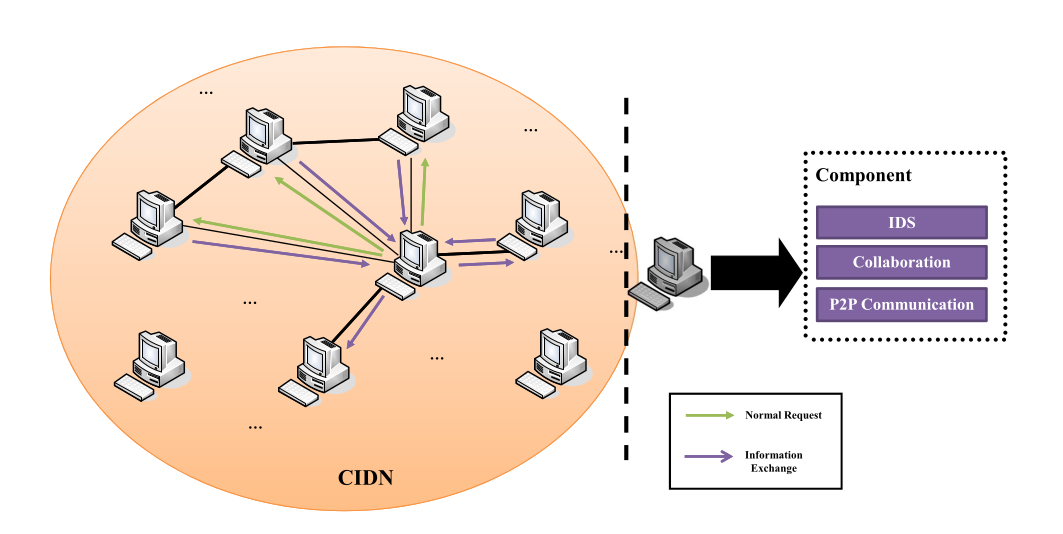
\includegraphics[width=.9\textwidth]{images/cids}
\caption{Dateien zur Erstellung des Templates}
\label{fig:templateprozess}
\end{figure}

Weitere separate Dateien sind die beiden Dateien mit 
den Literatur- und Online-Quellen 
\verb|thesis.bib| und \verb|online.bib|. \label{page:bib}
In \verb|thesis.bib| sollte die richtige Literatur sein, 
die gedruckt vorliegen kann beziehungsweise eine ISSN oder ISBN hat. 
In \verb|online.bib| werden Quellen, die ausschließlich Online verfügbar
sind gesammelt.  
Beim Referenzieren werden die beiden Quellen-Verzeichnisse automatisch
verwendet und später getrennt unter zwei Überschriften ausgewiesen. 
Zum Erstellen muss man je Datei separat \lstinline{bibtex} aufrufen. 
Wie schon in Abschnitt~\ref{sec:was} beschrieben braucht man zwei
Aufrufe um die Literaturreferenzen zu aktualisieren, welche steht
im \verb|Makefile|.
Eine beispielhafte Übersicht über die wichtigsten Quell-, 
Zwischen-, und Zieldateien finden Sie in 
Abbildung~\ref{fig:templateprozess}.


\chapter{Seitenlayout und Sprache} \label{chap:layout}
\epigraphhead[70]{\epigraph{I can’t go to a restaurant and 
order food because I keep looking at the fonts on the 
menu.}{\textit{Donald Knuth}}}

Das Seitenlayout des Templates sowie die Seitenmarkierungen
und die Schriften lassen einige wenige Wahlmöglichkeiten zu.
Es sollte so aufeinander abgestimmt sein, dass es ein 
angenehmes Erscheinungsbild ergibt.
Lassen Sie es so wie es ist und konzentrieren Sie sich auf
die Hinweise für das Schreiben in der deutschen Sprache.

\section{Papier und Abstände}

In \LaTeX\ sind für das Papierformat amerikanische Maße 
wie z.B. \verb|letter| vor\-ge\-ge\-ben. 
Es gibt jedoch für die im deutschen Raum üblichen Formate Vorlagen. 
Wir verwenden A4-Papier und passen die Abstände und Leerräume an.
Der Text hat eine Breite von 14~cm und eine Höhe von 22~cm.
Wir setzen den Text mittig mit einem Abstand am linken Rand von 
3,5~cm. 
Das Layout ist einseitig.
Drucken und binden Sie Ihre Abschlussarbeit auch einseitig.
Ändern Sie das Layout wenn irgend möglich nicht in ein doppelseitiges 
Layout.
Viele drucken dann falsch aus und ungerade Seiten sind dann nicht 
rechts.
Auch stimmen Abstände meist nicht, die alternierend gesetzt werden
müssten.
Des weiteren ist bei dem üblichen 80g-Papier der einseitige Druck 
angenehmer zu lesen, da dann weniger Inhalt durchscheint. 
Widerstehen Sie der Versuchung doppelseitigen Druck auf 120g Papier
durchzuziehen. 
Da Sie ja nicht sinnlos Seiten füllen sollen ist ein Umfang
der Abschlussarbeit mit 30--40 inhaltsschwangeren Seiten vollkommen 
in Ordnung. 
Wenn diese dann doppelseitig gedruckt in festen Einband gewickelt sind,
dann sehen diese 15--20 Blätter etwas komisch aus. 

Der Zeilenabstand wird mit 
(nicht mit \verb|baselinestretch| sondern) passenden Paketen 
auf das 1.15-fache des normalen Satzes gedehnt. 
Das ist für eine Abschlussarbeit angenehmer zu lesen und
entspricht grob der altertümlichen Vorgabe "`anderthalbzeilig"'.
Zusätzlich scheinen die meisten Menschen heutzutage einen Abstand
zwischen Absätzen zu bevorzugen. 
Wir nehmen hier 20 Prozent der Höhe des \verb|m| im 
verwendeten Zeichensatz.
Was bleibt ist das Einrücken Am Anfang des Absatzes mit Ausnahme des 
ersten Absatzes nach einer Überschrift.


\section{Seitenmarkierungen}

Als Seitenmarkierungen nehmen wir ausschließlich Markierungen
oben und lassen unten alles weg. 
Oben nehmen wir links die Kapitelüberschrift und rechts
die Seitennummer. 
Die Kapitelüberschrift wird in einer kleineren und 
serifenlosen Schrift gesetzt.
Auch wenn es vielleicht altbacken wirkt, so ist bei einer
Abschlussarbeit ein trennender Strich zwischen Kopf und 
Fließtext üblich.

Beim Kapitelanfang bleibt traditionell nichts oben stehen 
und die Seitenzahl mittig unten.
Es finden sich im Template auf der ersten Seite noch Zitate.
Es ist meist schwierig passende Zitate zu finden.
Verwenden Sie Ihre Zeit effektiver und lassen Sie die Zitate weg.


\section{Schriften}

Das Dokument soll sowohl beim Ausdruck als auch online in
PDF-Form gut aussehen. 
Das funktioniert nur mit Vektor-basierten Schriften beziehungsweise
Zeichensätzen, wie zum Beispiel den bei Postscript garantiert 
vorhandenen Schriften.
Bei \LaTeX\ kümmern sich darum die Pakete \verb|mathptmx| für
Times New Roman, \verb|helvet| für Helvetica (eine serifenlose
Schrift, an der man sich eigentlich auch schon satt gesehen 
hat) oder \verb|mathpazo| für Palatino. 
In diesem Dokument wird Palatino verwendet.
Hier können Sie sich jeweils einen Absatz in den unterschiedlichen 
Schriften anschauen.

\noindent\parbox[t]{\textwidth}{
\fontfamily{ptm}\fontsize{11}{13pt}\selectfont \ 
(Times New Roman) When Apollo Mission Astronaut Neil Armstrong first 
walked on the moon, he not only gave his famous ``one small step 
for man, one giant leap for mankind'' statement but followed it by 
several remarks, usual communication traffic between him, the other
astronauts and Mission Control. 
Just before he re-entered the lander, however, he made this 
remark \textit{Good luck Mr. Gorsky}.
}

\noindent\parbox[t]{\textwidth}{
\fontfamily{phv}\fontsize{11}{13pt}\selectfont \ 
(Helvetica) Many people at NASA thought it was a casual remark concerning 
some rival Soviet Cosmonaut. 
However, upon checking, there was no Gorsky in either the
Russian or American space programs. 
Over the years many people questioned Armstrong as to what 
the \textit{Good luck Mr. Gorsky} statement meant, but Armstrong
always just smiled.
On July 5, 1995 in Tampa Bay FL, while answering questions following 
a speech, a reporter brought up the 26 year old question to Armstrong. 
This time he finally responded. Mr. Gorsky had finally died and so 
Neil Armstrong felt he could answer the question.
}

\noindent\parbox[t]{\textwidth}{
\fontfamily{pplx}\fontsize{11}{13pt}\selectfont \ 
(Palatino) When he was a kid, he was playing baseball with a friend 
in the backyard. His friend hit a fly ball, which landed in the front 
of his neighbor's bedroom windows. 
His neighbors were Mr. \& Mrs. Gorsky.
As he leaned down to pick up the ball, young Armstrong heard 
Mrs.Gorsky shouting at Mr. Gorsky. 
\textit{Oral sex! You want oral sex?! You'll get oral sex when the 
  kid next door walks on the moon!}
}


\section{Sprache}

Sie schreiben Ihre Abschlussarbeit meist in Deutsch und
verwenden die neue deut\-sche Rechtschreibung.
Es ist natürlich möglich die Abschlussarbeit auch auf Englisch
zu schreiben, dazu muss das Template allerdings umgestellt werden. 
Im Folgenden gehen wir davon aus, dass Sie in Deutsch schreiben.
Korrekte Rechtschreibung und insbesondere korrekte Groß- und
Kleinschreibung werden gern gesehen, sogar das eine oder
andere Komma ist nicht zu verachten.
Auch bei Zwischenbesprechungen --- von denen es drei geben
sollte und bei denen \textbf{immer} Geschriebenes und
Gemaltes dabei ist --- sollte die Rechtschreibung schon passen.
Übrigens heißt es "`Standard"' und nicht "`\falsch{Standart}"'
und "`Zum einen \ldots und zum anderen \ldots"' und nicht 
"`zum \falsch{Einen}) \ldots und zum \falsch{Anderen}"'.

Schreiben Sie Zahlen von eins bis neun aus. Erst
ab der Zahl 10 verwenden Sie Ziffern. 
\falsch{Also nicht gleich 2 Fehler oder hundertunddreizehn Fehler
machen}.
Machen Sie Fußnoten\footnote{Das ist eine Fußnote.} immer
ohne einleitendes Leerzeichen und innerhalb des Satzes,
also nie nach einem Punkt. 
Fußnoten sind ganze Sätze mit Satzzeichen.
Fußnoten sind Inhalte, die nicht für das Verständnis 
notwendig sind\footnote{Fußnoten haben übrigens 
nichts mit Noten oder Musik zu tun.}. 
Juristen verwenden Fußnoten zur Quellenangabe. Wir
sind keine Juristen und distanzieren uns 
(nicht nur) von dieser Praxis deutlich.
Setzen Sie Fußnoten sehr sehr sparsam ein.

\falsch{Es gibt keine Abs\"{a}tze, die nur aus einem Satz bestehen.}

Schreiben Sie immer mehrere Sätze in einem Absatz. 
Falls nur ein Satz in einem Absatz ist irritiert das
den Leser. 
Außerdem sieht es sehr bescheiden aus.
Wenn es eigentlich gar nicht wichtig ist, dann lassen Sie 
den Satz weg. 
Wenn man es sagen muss, es aber nicht heraus stehen soll, dann
bringen Sie es in einem anderen Absatz unter. 
Wenn es wirklich wichtig ist, dann kann man auch drei Sätze 
dazu schreiben.

Referenzieren Sie innerhalb des Dokuments, zum Beispiel
auf das Kapitel~\ref{chap:bilder} in dem es unter anderem
um Bilder geht und das auf Seite~\pageref{chap:bilder}
los geht, mit \verb|\ref| (meistens) oder 
\verb|pageref| (sehr selten). 
Verwenden Sie vor dem Befehl zum Referenzieren immer
ein \verb|~|. Das ist ein nicht umbrechbares Leerzeichen
und \falsch{Kapitel \\ 1}, also der 
Zeilenumbruch vor der Nummerierung, wird vermieden.

\falsch{Es macht keinen Sinn aus irgendwelchen Gr"unden}\newline
\falsch{erscheinen sie noch so sinnvoll}\\ 
\falsch{Zeilenbr"uche im Flie"stext einzuf"uhren.}\\
\falsch{Sie}\\
\falsch{wollen eigentlich etwas anderes.}

Sie sollten Abkürzungen (AKÜ) bei ersten Vorkommen definieren.
Schreiben Sie das Wort zuerst aus und dann die Abkürzung in 
Klammern. 
Danach können Sie die AKÜ verwenden. 
Meistens sollten Sie jedoch auf Abkürzungen verzichten.
Schreiben Sie lieber
\textit{beispielsweise, zum Beispiel, und so weiter, beziehungsweise}
statt \textit{bspw., z.B., usw., bzw.}.

Setzen Sie die drei verschiedenen Bindestriche -, -- und --- richtig
ein. 
Der einfache Bindestrich - wird bei Worttrennungen, 
wie AKÜ-Fimmel, eingesetzt (im Quelltext mit \verb|-|).
Der etwas längere Streckenstrich -- wird bei Streckenangaben, wie
die Strecke Wiesbaden--Frankfurt oder von 10:00--11:45 eingesetzt
(im Quelltext mit \verb|--|).
Der Gedankenstrich --- ist bei Einschüben --- wie zum Beispiel
hier --- einzusetzen (im Quelltext mit \verb|---|).
\falsch{Es ist auf keinen Fall ein Leerzeichen um einen Binde - strich 
oder einen Strecken -- strich und immer ein Leerzeichen
um einen Gedanken---strich}.

\chapter{Bilder und Listings} \label{chap:bilder}
\epigraphhead[70]{\epigraph{I have always wished for my computer to be 
as easy to use as my telephone; my wish has come true because I can no 
longer figure out how to use my telephone.}{\textit{Bjarne Stroustrup}}}

Bilder werden meist unabhängig von \LaTeX\ erstellt und dann nur 
eingebunden. 
Bilder, genau wie Tabellen, Listings oder ähnliches, sind dabei nicht 
Teil des normalen Fließtexts sondern separate Objekte, 
deren Position sich nach Gutdünken des Setzers (also \LaTeX) 
ändern kann.
Diese fließenden Objekte, oder auch Fließobjekte,
beinhalten dann das Bild, das Listing oder die Tabelle.


\section{Fließobjekte}

Bilder, Listings und Tabellen sollten als Fließobjekte (\emph{floats}) 
oder Float-Objekte gesetzt werden.
Das heißt \LaTeX\ entscheidet wohin das Objekt kommt, man selbst
gibt nur Hinweise wo es gut wäre.
Fließobjekte wie zum Beispiel Tabelle~\ref{tab:meinetab} müssen immer im 
Text referenziert werden.

\begin{table}[htbp] % htbp ~ here, top, bottom, page
\centering
\begin{tabular}{|r|c|l|l|}
\hline
\textbf{Name} & \textbf{Adresse} & \textbf{Wohnort} & \textbf{Telefon} \\ 
\hline\hline
Susi Sinnlos & Eichenstrasse 5 & 12345 Unterstadt & 24927749242 \\
Horst Kurz & Schnellweg 17 & 42420 Rapid & 999 \\\hline
Jochanaan Leuchtentrager & Hochstraße zu & 666 Hell & 1-800-33845\\\hline
\end{tabular}
\caption{Adressliste}
\label{tab:meinetab}
\end{table}

Die entsprechenden vordefinierten Umgebungen heißen 
\verb|table| für Tabellen und \verb|figure| für Abbildungen. 
Mit den optionalen Argumenten \verb|htbp|, das steht für
\textit{here, top, bottom, page}, geben Sie \LaTeX\ den 
Tipp, dass Sie am liebsten das Fließobjekt \textit{hier}
an dieser Stelle haben möchten. Wenn das nicht geht, dann
eben am \textit{Anfang} der Seite, und wenn das nicht geht (weil es
zum Beispiel ein Kapitelanfang ist) ans \textit{Ende} der Seite. 
Wenn das alles nicht klappt, dann halt auf eine Extra-\textit{Seite}.
Beherzigen Sie folgende Tipps zu Fließobjekten:
\begin{itemize}
\item Jede Tabelle, jedes Bild und jedes Listing ist ein Fließobjekt.
\item Zentrieren Sie Bilder und Tabellen.
\item Jedes Fließobjekt hat eine Bildunterschrift (Caption) mit
  einem Label und wird im Text passend referenziert.
\end{itemize}
Schreiben Sie nie, \falsch{wie man unten in der Tabelle sehen kann},
da Sie nie wissen und auch nicht wissen sollen, ob die Tabelle 
wirklich \glqq weiter unten\grqq\ ist. 
Verwenden Sie statt relativer Positionsangaben Referenzen mit Zahlen,
die Sie durch das Label erhalten, wie zum Beispiel 
"`wie sie in Tabelle~\ref{tab:meinetab} sehen können"'.
Verwenden Sie kurze und prägnante Bildunterschriften, die 
nicht länger als eine Zeile lang sind. 
Alles was mehr als eine Zeile hat gehört in den Fließtext.
Sie sollten für die Fließobjekt Caption keinen Satz bilden und 
daher auch keinen Punkt am Ende haben.
Die Caption ist eine Unterschrift und gehört unter das Fließobjekt.

\begin{wrapfigure}{r}{6cm}
  \centering
  
\includegraphics[width=4cm]{images/gnu}
  \caption{GNU-Logo~\cite{images/gnulogo,fal}}
  \label{fig:gnu}
\end{wrapfigure}
Es ist möglich, wenn auch nicht empfohlen, 
Bilder an den 
Rand einer Seite zu klatschen, wie wir das mit dem 
GNU-Logo in Abbildung~\ref{fig:gnu} gemacht haben. 
Das ganze ist ein netter Effekt für Graphiken, wie zum Beispiel ein
Logo, die nicht zum Verständnis des Texts gebraucht werden und wenig
Details aufweisen. 
Der Effekt sollte aber nicht überstrapaziert werden, 1--2 Mal 
je Abschlussarbeit sollte, wenn überhaupt, rei\-chen.
Außerdem funktioniert \verb|wrapfigure| nicht immer sehr stabil.

\section{Bilder}

Neben einer Tabelle~\cite{kopka}, wie in Tabelle~\ref{tab:meinetab},
kann man auch eine Bild oder Grafik als Fließobjekt einsetzen.
Man nimmt mit PDFLaTeX entweder ein PDF für Vektorgrafiken,
ein JPG für Photographien und ein PNG für Bilder mit gleichfarbigen
Flächen, wie zum Beispiel Screenshots.
Bitte nehmen Sie \textbf{nie} JPG oder PNG für Vektorgrafiken, 
also Zeichnungen mit Linien oder anderen geometrischen Objekten,
sondern ausschließlich PDF.
Binden Sie also \textbf{nie} Vektorgraphiken verpixelt ein.
In Abbildung~\ref{fig:tk} finden Sie eine große Konzeptzeichnung, 
die skaliert wurde um den Platz vollständig auszufüllen. 
\begin{figure}[htb]
\centering
%\includegraphics[width=.6\textwidth]{zeichnung} % pdflatex ohne Endung
\caption{Die tolle Konzeptzeichnung}
\label{fig:tk}
\end{figure}
Die Grafik wurde mit LibreOffice~\cite{libreoffice} erstellt. 
Die Draw-Komponente erlaubt es recht einfach Vektorgrafiken zu 
erstellen und in PDF-Format zu wandeln. 
Mit LibreOffice geht das sogar von der Kommandozeile und damit
von einem Makefile aus.

Man kann auch zwei Grafiken nebeneinander einbinden wie es in 
Abbildung~\ref{fig:tk2} passiert ist. 
Machen Sie sich klar, dass man immer nur Abbildung~\ref{fig:vektor}
haben will und \textbf{nie} 
Abbildung~\ref{fig:jpg} oder~\ref{fig:png}, 
da diese verpixelte Bilder einer Vektorgrafik sind.

Es empfiehlt sich, die Grafiken alle in einer einheitlichen Größe
zu erstellen und dann unskaliert oder immer mit der gleichen 
Skalierung einzubinden. 
Nur dann sind auch die verwendeten Schriften nicht skaliert, sondern 
in der geplanten Größe. 
Verwenden Sie wenn möglich einen der Standardschriften von Postscript 
in den Vektorgrafiken.

\begin{figure}[htb]
\centering
\subfloat[Vektor]{\label{fig:vektor}
  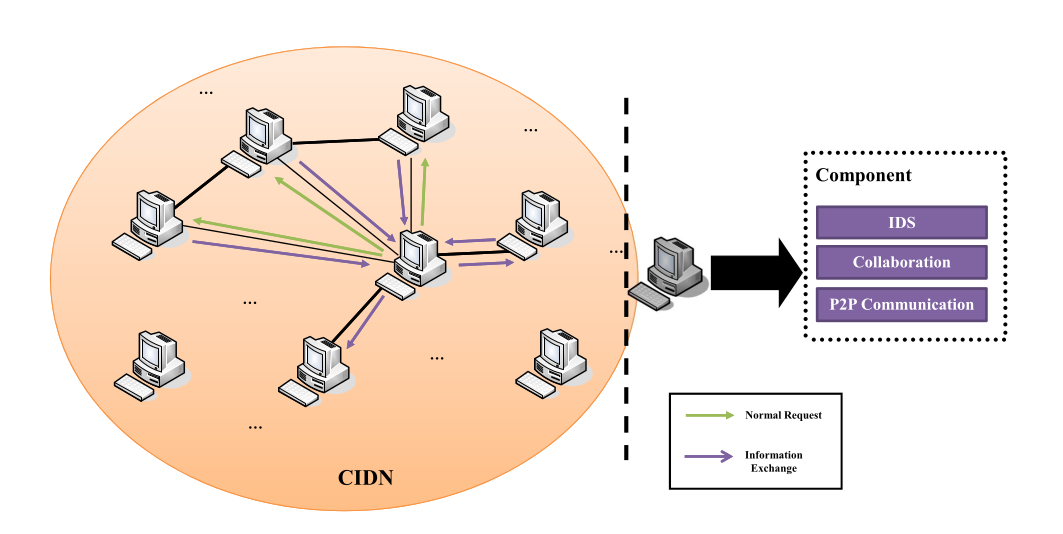
\includegraphics[width=.3\textwidth]{images/cids}}
\subfloat[JPG]{\label{fig:jpg}
  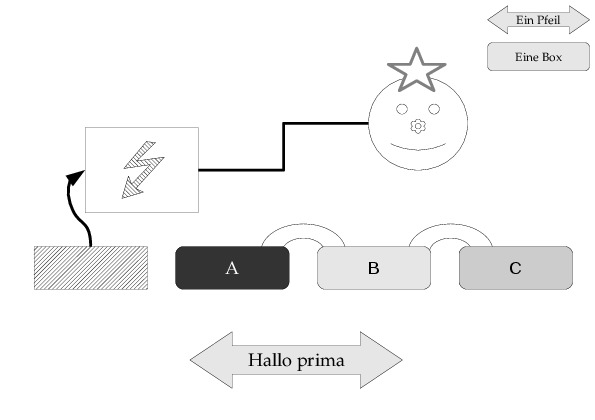
\includegraphics[width=.3\textwidth]{images/zeichnungjpg}}
\subfloat[PNG]{\label{fig:png}
  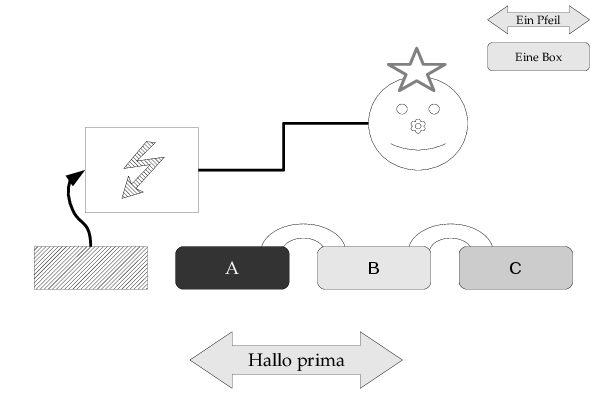
\includegraphics[width=.3\textwidth]{images/zeichnungpng}}
\caption{Die tolle Konzeptzeichnung in unterschiedlichen Formaten}
\label{fig:tk2}
\end{figure}

Es ist durchaus in Ordnung und vermutlich recht schlau, wenn Sie initial 
die Bilder mit der Hand zeichnen und mit einer Kamera abfotografieren. 
Für die tolle Konzeptzeichnung ist ein Beispiel in 
Abbildung~\ref{fig:tkdraft} zu finden. 
Damit vermeiden Sie eine Ablenkung durch Tools und konzentrieren
sich auf die Inhalte. 
Die eigentlichen Vektorgrafiken können Sie dann entspannt kurz vor
der Abgabe in einer Session erledigen. 

\begin{figure}[htb]
\centering
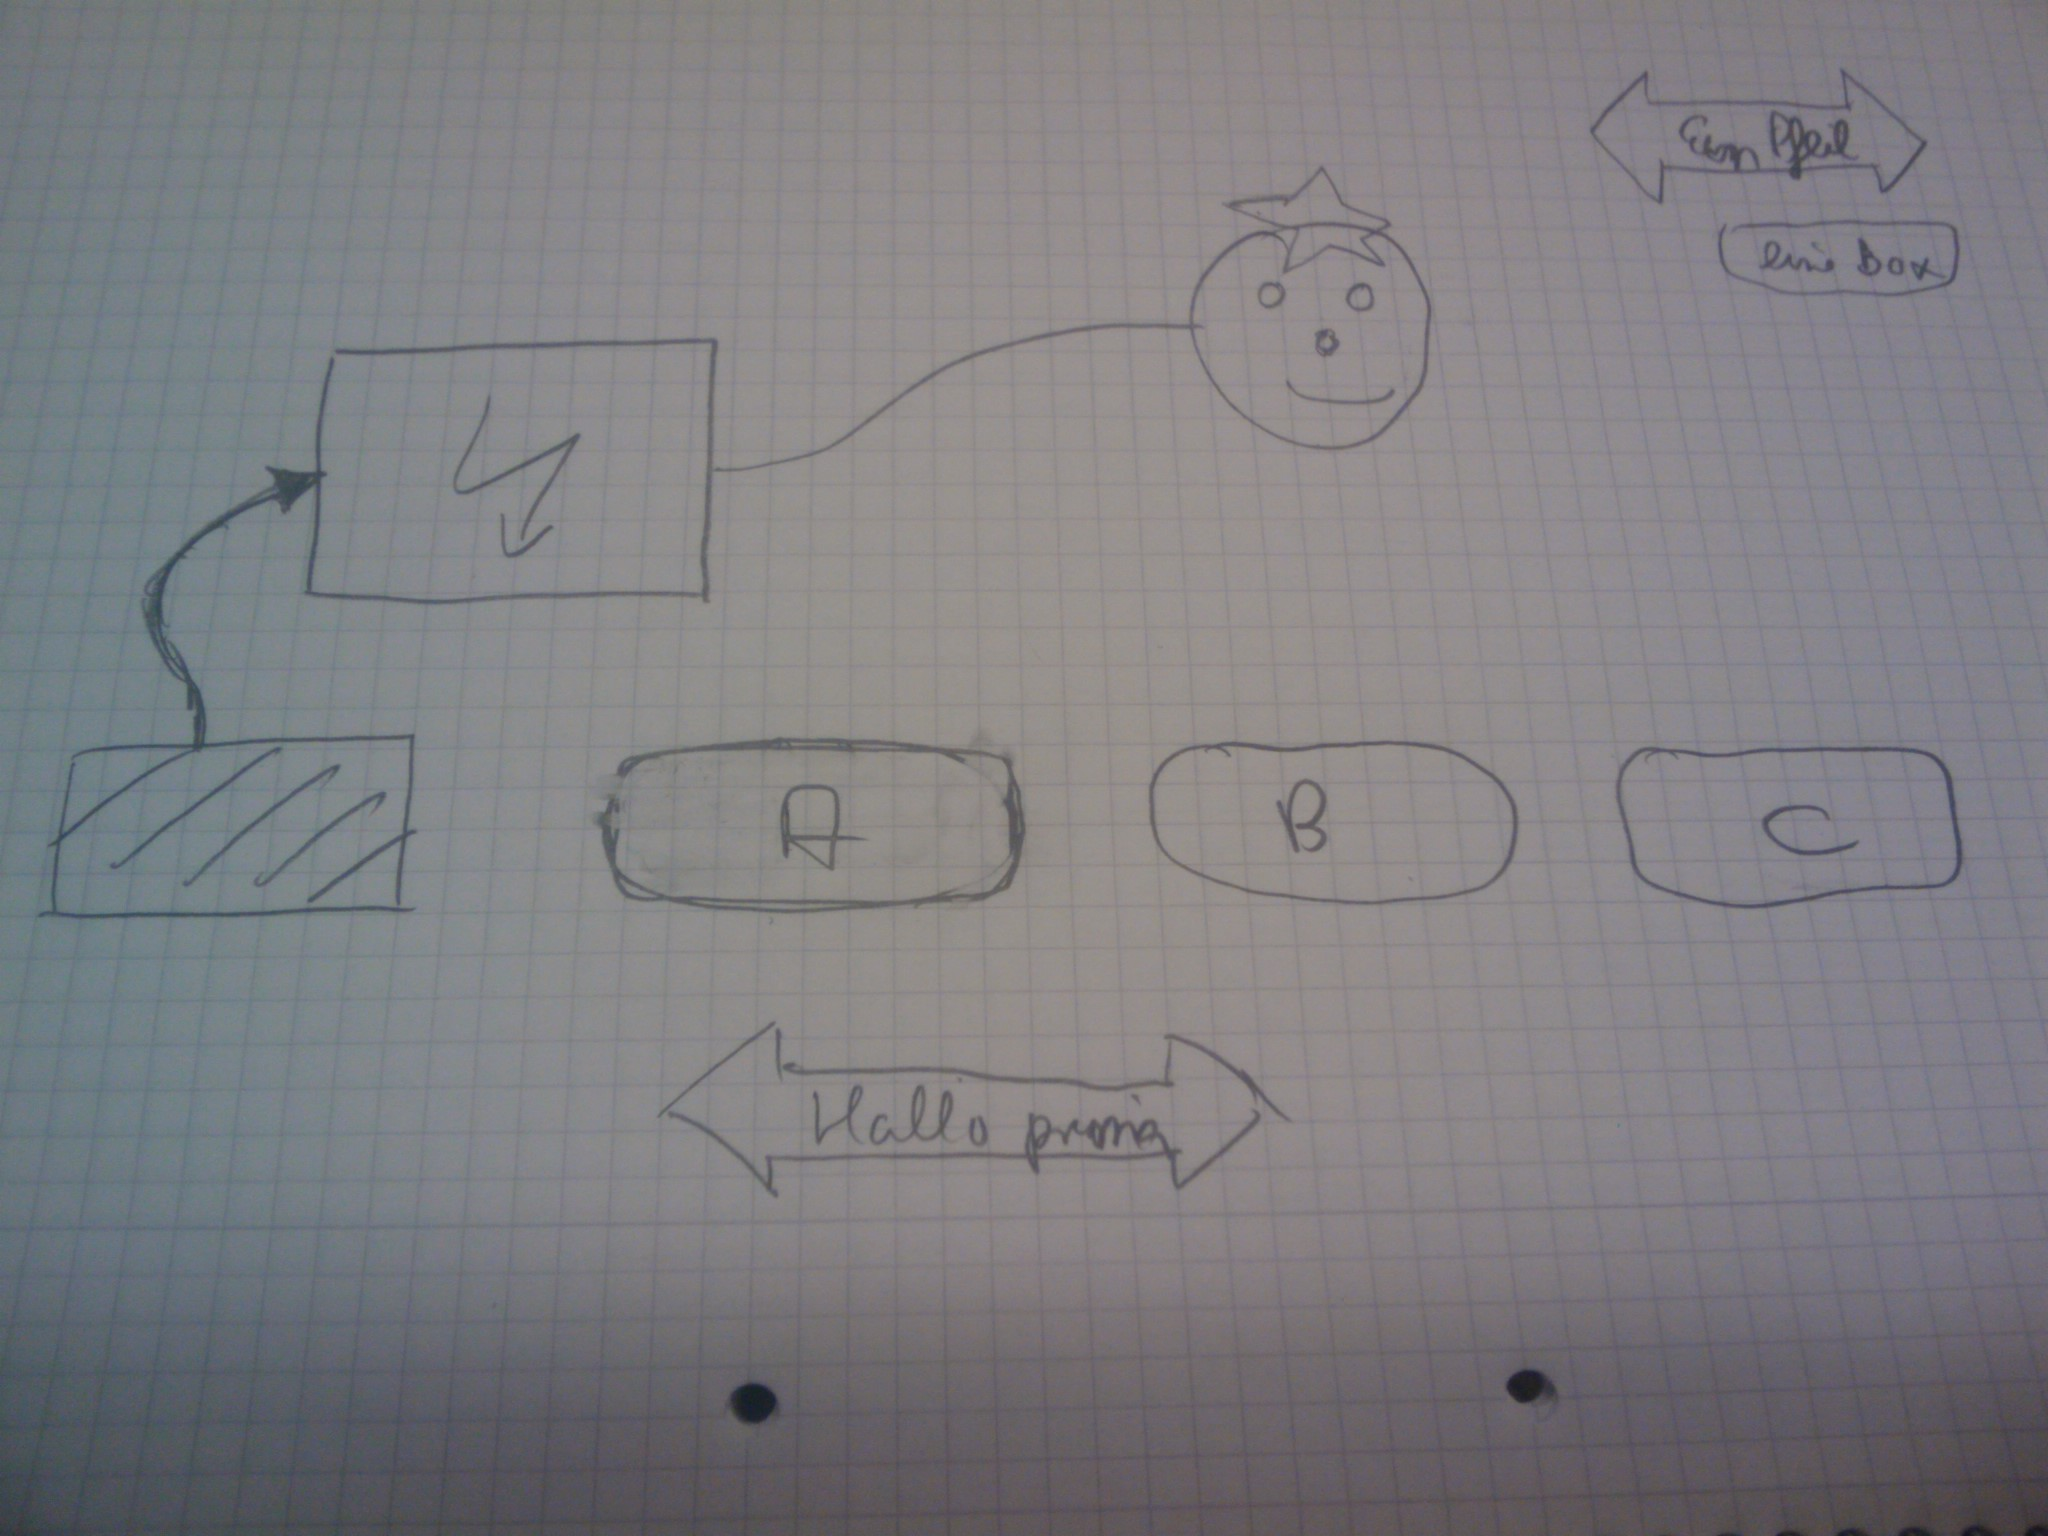
\includegraphics[width=.4\textwidth]{images/zeichnungdraft} 
\caption{Die tolle Konzeptzeichnung als Draft}
\label{fig:tkdraft}
\end{figure}

Auch wenn es hart erscheint: Vermeiden Sie Farben. 
Sie machen meist Konzeptzeichnungen und benötigen keine Farben. 
Wenn Sie Farben einsetzen, dann müssen Sie sehr intensiv
über einen sinnvollen Einsatz nachdenken. 
Häufig endet das aber nur damit, dass man ein paar potenziell wichtige Sachen
bunt macht; das hilft nicht. 
Mit Graustufen und Schraffierungen kommen Sie recht weit und
die sind erlaubt. 
Der Vorteil ist, dass Sie auf einen hochauflösendem Drucker
schnell eine sehr gute Qualität erzielen und notfalls das 
ganze schnell ausgedruckt haben. 
Eine Ausnahme sind natürlich Abschlussarbeiten wo Farben 
essentiell sind. 
Wenn Sie zum Beispiel Bildverarbeitung machen und haben 
farbige Bilder als Ausgangsmaterial ist es natürlich sinnvoll
die Abschlussarbeit bunt zu machen. 
Auch andere "`Ausreden"' Abschlussarbeiten bunt zu machen 
werden akzeptiert.
Aber spätestens bei farbigen deckenden Abbildungen tun Sie sich 
und den Lesern den Gefallen und drucken Sie Ihre Arbeit einseitig aus.

Wer will, der kann auch mit \LaTeX\ direkt Grafiken 
erstellen~\cite{kopka}.
Das ist jedoch nur etwas für Hartgesottene.
Eine attraktivere Variante ist PGF und TikZ~\cite{tikz}.
In Abbildung~\ref{fig:tikz} ist ein Beispiel eines direkt mit 
TikZ erzeugter Graphik. 

\begin{figure}[htb]
\centering
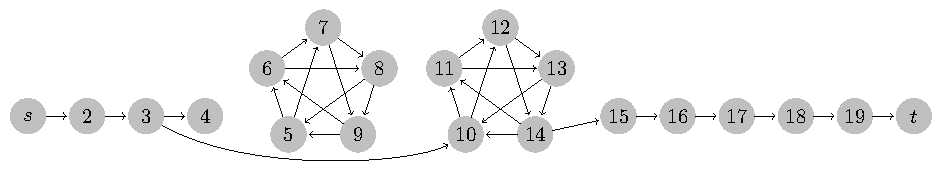
\includegraphics[width=.9\textwidth]{automata} % pdflatex ohne Endung
\caption{Automaten mit tikz~\cite{tikzautomata}}
\label{fig:tikz}
\end{figure}

Damit dieses Template nicht die Installation von TikZ voraussetzt
ist hier nur das PDF eingebunden. 
Wer professionell Abbildungen setzen will, der sollte sich das aber
mal anschauen.


\section{Listings} \label{sec:listings}

Am einfachsten und meist am sinnvollsten ist es keine
Listings in Ihrer Arbeit abzudrucken. 
Falls Sie doch davon nicht abzubringen sind, dann 
machen Sie sich klar, dass fast ohne Ausnahme Listings
auch immer Fließobjekte sind, wie zum Beispiel ein
sehr ausführlicher langsamer größter gemeinsamer Teiler (ggT) 
in Listing~\ref{code:ggtaua}.
Vermeiden Sie solche langen Listings.

\begin{listing}[ht]
\begin{lstlisting}
def ggt(x, y):
    if x == y or x == 1 or y == 1:
        return min(x,y)
    if x > y:
        x,y = y,x
    # es gilt x < y
    return ggt(x, y-x)
\end{lstlisting}
\caption{ggT --- lang und schlecht}
\label{code:ggtaua}
\end{listing}

Neben langen Listings sind natürlich kurze prägnante
Listings in Pseudocode (oder Python ;-) viel 
angenehmener, wie in Listing~\ref{code:ggt} der
effiziente GGT.

\begin{listing}[htbp]
\begin{lstlisting}
def ggt(x, y):
    while x != 0:
        x,y = y%x, x
    return y
\end{lstlisting}
\caption{ggT --- kurz und gut}
\label{code:ggt}
\end{listing}

Die Parameter für Listings sollte man für das ganze Dokument gleich 
lassen. 
Wenn man mal unbedingt wechseln will, dann ist das auch möglich,
wie zum Beispiel bei Listing~\ref{code:ggtjava}, das den ggT
in Java mit einem anderen Zeichensatz zeigt.

\begin{listing}[htbp]
\lstset{basicstyle=\sffamily, columns=[l]flexible, mathescape=true, showstringspaces=true, numbers=none, language=java}
\begin{lstlisting}
public static int ggt(int x, int y) {
    while (x != 0) {
        int h = x;
        x = y%x;
        y = h;
    }
    return y;
}
\end{lstlisting}
\caption{ggT --- Java}
\label{code:ggtjava}
\end{listing}

Der verwendete serifenlose Zeichensatz sieht vielleicht schöner 
aus, aber der variable Zeichenabstand kann bei Listing störend 
sein. Der in den Beispielen Listing~\ref{code:ggtaua} und 
Listing~\ref{code:ggt} verwendete Zeichensatz mit festem
Zeichenabstand ist für Quellcode meist zu bevorzugen.

Sie sollten nie mit einem Listing oder einem anderen Fließobjekt 
einen Abschnitt beenden. 
Schreiben Sie noch etwas, 
notfalls einen Hinweis auf den nächsten Abschnitt.

\chapter{Hinweise} \label{chap:stil}
\epigraphhead[70]{\epigraph{Those are my principles, 
and if you don't like them...\newline
well, I have others.}{\textit{Groucho Marx}}}

Ihr Schreibstil, wann Sie mathematische Formeln verwenden
und was Sie zitieren ist individuell unterschiedlich.
Anbei eine Sammlung persönlicher Präferenzen zusammen mit 
einer (hoffentlich) korrekten Umsetzung.


\section{Schreibstil} \label{sec:schreibstil}

Schreiben Sie kurze, verständliche Sätze.
Blasen Sie Ihre Arbeit nicht auf um Seiten zu schinden.
Beschreiben Sie Ergebnisse und vermeiden Sie Schilderungen
Ihrer Arbeitsprozesse sowie Allgemeinplätze. 
Schreiben Sie nicht in Ich-Perspektive.
\falsch{Ich habe bei Besprechungen mit Studierenden
festgestellt, dass viele Sachen bei einer Abschlussarbeit falsch gemacht 
werden. 
Um dem vorzubeugen gibt es hier ein Template das Sie verwenden k"{o}nnen. 
Die Hinweise darin sind wichtig und sollten befolgt werden.
Ich denke schon, dass es Sinn macht die Hinweise zu lesen und 
zumindest eine Begr\"{u}ndung zu haben, wenn man sich nicht daran 
h\"{a}lt.}

Idealerweise verwenden Sie spätestens jede zweite Seite ein Bild. 
Ein Bild lockert auf und "`sagt mehr als tausend Worte"'.
Vermeiden Sie Aufzählungen. 
Aufzählungen brauchen meist viel Platz und ersetzen häufig 
eine viel besser passende Tabelle. 
Idealerweise haben Sie Aufzählungen nur an einer oder
zwei Stellen, zum Beispiel am Anfang der Arbeit um Ihre
Aufgabenstellung klar aufzuschreiben. 
Sie schreiben Fließtext und pressen nicht eine Powerpoint
Präsentation in \LaTeX.
Aufzählungen bestehen meist aus drei Punkten und wenn 
es Unterpunkt gibt, dann wieder aus drei Unterpunkten.
Punkte in Aufzählungen bestehen nur aus wenigen Zeilen.
Wenn es länger wird, dann wollten Sie vielleicht einen
Absatz schreiben.

Verwenden Sie niemals zwei hintereinander folgende Überschriften.
Es muss immer etwas zwischen zwei Überschriften stehen. 
Idealerweise geben die kurzen Absätze beziehungsweise Paragrafen 
nach jeder Hauptüberschrift eine gute Zusammenfassung der Arbeit 
(Ergebnisse, nicht Vorgehen).
Absätze bestehen immer aus mehr als einem Satz. 
Idealerweise mindestens drei Sätze und mindestens vier 
Zeilen\footnote{
Die konkreten Zahlen sind nicht bindend. 
Sie werden hier nur genannt, weil man ansonsten immer 
danach gefragt wird. 
}.

Lesen Sie Literatur zum technischen Schreiben~\cite{gockel,rechenberg}.
Die beiden Bücher sind verständlich geschrieben und enthalten
neben allgemeinen Ratschlägen auch konkrete Hinweise, Hilfen und
Beispiele.


\section{Mathematik} \label{sec:mathematik}

\LaTeX\ ist sehr gut geeignet Formeln zu setzen und 
allgemein beliebige Themen formal aufzuschreiben.
Sie können also gerne mathematische Formeln in Ihrer 
Abschlussarbeit verwenden, aber achten Sie darauf, dass
es Sinn macht. 
Beim Textsatz mathematischer Formeln sollten Sie zwischen 
Formeln innerhalb einer Zeile und abgesetzten Formeln unterscheiden. 
Abgesetzte Formeln können zusätzlich noch einfach referenzierbar
gemacht werden.

Eine Formel kann im Fließtext integriert sein, wie zum Beispiel 
$\sum_{i=1}^n i = \frac{n \cdot (n+1)}{2}$ oder separat
und referenzierbar gesetzt werden wie die Folgende:
\begin{equation} \label{eq:gauss}
  \sum_{i=1}^n i = \frac{n \cdot (n+1)}{2}
\end{equation}
Im \LaTeX-Quelltext werden beide Arten von Formeln gleich geschrieben 
aber anders gesetzt. 
Achten Sie zum Beispiel auf das Summenzeichen und die Positionen 
des Index. 
Die Gleichung~\ref{eq:gauss} ist natürlich vom Fließtext aus referenzierbar.
Man kann auch schreiben: 
(\ref{eq:gauss}) ist natürlich vom Fließtext aus referenzierbar.
Im Fließtext kann man auch gerne auf den Bruch verzichten und 
$\sum_{i=1}^n i = (n \cdot (n+1))/2$
schreiben, was meist etwas lesbarer ist.
Alternativ geht auch 
$\sum_{i=1}^n i = \mbox{\textonehalf} \cdot n \cdot (n+1)$.
Achten Sie bei Formeln darauf als Multiplikationszeichen 
$\cdot$ zu verwenden und nicht $*$. 
Ich kenne einen Kollegen, der ansonsten dadurch sehr erregt wird. 

Sie können viele Symbole, wie die griechischen Buchstaben 
$\alpha, \beta, \gamma, \ldots$;
logische Symbole wie $\forall, \exists, \not\exists, \wedge, \vee, \neg,
\Rightarrow, \Leftrightarrow$;
Mengensymbole wie $\in, \cup, \cap, \subseteq, \not\supset, 
\biguplus, \ldots$;
andere Symbole $\rightarrow, \sqsubseteq, \sim, 
\models, \vdash, \infty, \emptyset, \mathbb{N}, \mathbb{R}, \ldots$;
oder zusammengesetzte Gleichungen 
wie die Definition der 91er-Funktion~\cite{manna70}
verwenden.
\[
  f(x) = \left\{ \begin{array}{lll}
      x-10 & \mbox{gdw} & x>100 \\
      f(f(x+11)) & \multicolumn{2}{l}{\mbox{sonst}} 
    \end{array} \right.
\]
Viele weitere Beispiele finden Sie im Kopka~\cite{kopka}.
Falls diese nicht ausreichen können Sie eines der vielen
Erweiterungspakete verwenden, die Ihnen alle möglichen 
weiteren Symbole zur Verfügung stellen.

Nicht nur für reine Mathematik, sondern für jede formale
Darstellung kann es sinnvoll sein die klassische Aufteilung
von \emph{Definition}, \emph{Satz} und \emph{Beweis}
zu verwenden. 
Die drei Klassiker sind in \LaTeX\ in der Theorem-Umgebung 
vordefiniert und einfach zu verwenden.
Die Kapitel gehen in die Nummerierung mit ein.

\begin{definition}
Sei $\varepsilon = 0$.
\end{definition}

\begin{satz}
Für alle positiven ganzen Zahlen $n$ gilt 
$\sum_{i=1}^n i = \frac{n \cdot (n+1)}{2}$ \enspace.
\end{satz}
\begin{beweis}
Vollständige Induktion:
\begin{itemize}
\item \emph{Induktionsanfang ($n=1$):} Es gilt  
\[
  \sum_{i=1}^1 i \, = \, 1 \, = \, \frac{1 \cdot (1+1)}{2}.
\]
\item \emph{Induktionsschritt ($n \rightarrow n+1)$:}
Es gelte die Induktionsvoraussetzung (IV):
\[
\sum_{i=1}^n i = \frac{n \cdot (n+1)}{2}
\]
Wir zeigen, dass dann auch 
\[
\sum_{i=1}^{n+1} i = \frac{(n+1) \cdot (n+2)}{2}
\]
gilt wie folgt:
\begin{eqnarray*}
  \sum_{i=1}^{n+1} i 
  & = & (\sum_{i=1}^{n} i) + (n+1)  \\
  & =_{\mbox{IV}} & \frac{n \cdot (n+1)}{2} + (n+1) \\
  & = & \frac{n \cdot (n+1)}{2} + \frac{2 \cdot (n+1)}{2} \\
  & = & \frac{n \cdot (n+1) + 2 \cdot (n+1)}{2} \\
  & = & \frac{(n+2) \cdot (n+1)}{2} 
\end{eqnarray*}
\end{itemize}
\qed
\end{beweis}
Sie müssen den Dreisatz 
\emph{Definition}, \emph{Satz} und \emph{Beweis} nicht verwenden, 
wenn Sie kein sehr formales Thema haben. 
Eine sehr formale Aufarbeitung von bekanntem Inhalt gefolgt 
von einem nicht so formalen eigenen Anteil sollte man 
meist vermeiden.


\section{Literatur}

Für Ihre Abschlussarbeit werden Sie ordentlich recherchieren
und gefundene und verwendete Quellen sauber belegen. 
Das macht man durch die Angabe von Quellen, die im laufenden 
Text referenziert werden und am Ende der Arbeit in einem
separaten Verzeichnis gelistet werden. 
Wir zitieren \textbf{nicht} durch die Angabe von Quellen
in Fußnoten, das machen Juristen und Geisteswissenschaftler.

Bei den Quellen unterscheiden wir dabei zwischen Literatur und 
Online-Quellen.
Literatur ist etwas was in gedruckter Form vorliegen kann
und einen Eintrag in einem einschlägigen Verzeichnis hat,
also zum Beispiel eine ISBN oder ISSN hat.
Auch wenn Sie selbst das jeweilige Dokument nur elektronisch 
vorliegen haben, 
da Sie zum Beispiel den innerhalb der Hochschule angebotenen
Online-Dienst von ACM~\cite{acm} und IEEE~\cite{ieee} nutzen,
ist das kein Grund die Quelle unter Online-Quellen einzustufen.
Online-Quellen sind Quellen, die ausschließlich elektronisch
vorliegen. 
Dies könnten zum Beispiel Websites von Tools sein, so wie
in diesem Dokument vielfach verwendet. 
Bei Online-Quellen dokumentieren Sie den letzten erfolgreichen
Zugriff auf die Quelle.
Artikel aus Wikipedia~\cite{wikipedia} sind auch Online-Quellen.
Versuchen Sie auf Zitate aus Wikipedia zu verzichten. 
Es gibt zu den Themen für die Sie Wikipedia verwenden meist 
auch Literatur.
Wenn Sie denken es muss sein, dann zitieren Sie Wikipedia 
zumindest richtig~\cite{wikiciting}.
Versuchen Sie im Allgemeinen Online-Quellen nur dann einzusetzen
wenn es Sinn macht und keine Literatur vorhanden ist. 
Lesen Sie auch die Websites der Tools, die Sie einsetzen. 
Häufig schlagen die Autoren vor, wie zitiert werden soll.
So sollte man zum Beispiel für die LIBSVM~\cite{libsvm}
nicht die Online-Quelle, also die Website
\url{http://www.csie.ntu.edu.tw/~cjlin/libsvm/}, 
sondern einen passenden publizierten Artikel zitieren.

Bei den Literaturangaben hilft Ihnen \LaTeX\ zusammen mit
BiBTeX~\cite{bibtexing,kopka} ungemein.
Achten Sie übrigens darauf, dass mehrere Referenzen 
an einer Stelle zusammengeschrieben werden~\cite{bibtexing,kopka}
und \st{nicht auseinander~\mbox{\cite{bibtexing}}\mbox{~\cite{kopka}}}.
Die eigentlichen Informationen zu den Quellen werden 
in Dateien mit der Endung \verb|.bib| ausgelagert,
wie schon in Abschnitt~\ref{sec:template} 
auf Seite~\pageref{page:bib} beschrieben.
Einträge erhält man entweder direkt von einschlägigen
Suchdiensten wie zum Beispiel ACM~\cite{acm} oder
man legt sie selbst an.
Im Fließtext verwendet man \verb|\cite| mit dem Schlüssel
des jeweiligen Eintrags. 
Mehr ist in den \LaTeX-Quellen nicht zu machen. 
Wenn man die Literaturangaben ändert, dann muss
man erst \verb|thesis.tex| übersetzen.
Danach müssen Änderungen aus beiden \verb|.bib|-Dateien 
in das Dokument integriert werden. 
Auf der Konsole geht das wie folgt.
\begin{verbatim}
$ bibtex thesis1
$ bibtex thesis2
\end{verbatim}
Der erste Befehl extrahiert alles was aus \verb|thesis.bib|
referenziert wurde, der zweite Befehl extrahiert alles was aus 
\verb|online.bib| referenziert wurde, 
da wir die Verzeichnisse in der Reihenfolge eingebunden haben 
und \verb|thesis.tex| der Name des Hauptdokuments ist.
Häufig schaffen es IDEs nicht das automatisch richtig zu machen. 
Nach dem Lauf mit \verb|bibtex| sollte man noch einmal 
das \verb|.pdf| erzeugen, da ja die Literatur neu eingebunden
wird. Wenn Sie dabei wieder Seiten verschieben muss noch 
ein weiteres Mal \verb|pdflatex| ausgeführt werden. 


\chapter{Zusammenfassung und Ausblick} \label{chap:fazit}

Mit \LaTeX\ die Abschlussarbeit zu schreiben ist 
einfach und ergibt ein schönes, hochqualitatives Dokument.
Die Umgebung ist kostenlos und steht auf allen wichtigen
Plattformen zur Verfügung.
Im Gegensatz zu anderen Tools kann man sich beim Schreiben 
auf den Inhalt konzentrieren und steht großen Änderungen 
nicht ängstlich gegenüber.

Die Stärken von \LaTeX\ sind das Schreiben des Fließtexts
durch die Angabe von Struktur. 
Referenzieren innerhalb des Dokuments und auch auf 
Literatur sind sehr einfach und vollständig automatisiert. 
Selbst wenn die Erstellung von Bildern innerhalb von
\LaTeX\ auch möglich ist, verwenden viele lieber externe 
Tools für die Grafiken und binden diese dann ein. 
Auch dies wird sehr gut unterstützt und diese und
weitere Elemente wie Listings und Tabellen werden
von \LaTeX\ an eine passende Stelle gesetzt.

Das vorliegende Template vereinfacht die Erstellung
einer Abschlussarbeit an der Hochschule~RheinMain,
da formale Vorgaben an eine solche Abschlussarbeit
umgesetzt sind. 
Darüber hinaus ist das Template jedoch geprägt von 
persönlichen Vorlieben des Referenten. 
Diese persönlichen Vorlieben können Sie jedoch 
nach eingehender Beschäftigung mit \LaTeX\ auch gerne 
anders ausgestalten und einen eigenen Stil entwickeln.

Happy \TeX ing! 

\newpage

% Listen wenn überhaupt ans Ende und nicht an den Anfang.
% Meist ist das aber unnötig.
%\listoffigures % Liste der Abbildungen 
%\listoftables % Liste der Tabellen
% \newpage

\bibliographystyle{plain} % Literaturverzeichnis
\begin{btSect}{thesis} % mit bibtopic Quellen trennen
\section*{Literaturverzeichnis}
\btPrintCited
\end{btSect}
\begin{btSect}{online}
\section*{Online-Quellen}
\btPrintCited
\end{btSect}
% dann mit "bibtex thesis1" und "bibtex thesis2" arbeiten

\end{document}
;;; Local Variables:
;;; ispell-local-dictionary: "de_DE-neu"
;;; End:
